\documentclass{article}
\usepackage{framed}
\usepackage{scrextend}
\usepackage{xcolor}
\definecolor{shadecolor}{RGB}{105, 48, 195}
\usepackage[spanish,es-tabla]{babel}
\usepackage[dvips,a3paper,centering,margin=2cm]{geometry}
\usepackage{multicol}
\usepackage[utf8]{inputenc}
\usepackage{color}
\usepackage{float}
\usepackage{colortbl}
\usepackage{tabulary}
\usepackage{multirow}
\usepackage{amsmath}
\definecolor{rb}{rgb}{0.025,0.5,0.9} 
\definecolor{na}{RGB}{255,255,255}
\definecolor{title}{RGB}{55, 0, 49}
\usepackage{graphicx}  
\pagestyle{empty}
\def\to{\rightarrow}
\begin{document}
\vspace*{-2cm}
\changefontsizes{14pt}
\hspace*{-1cm}
\begin{minipage}{0.2\linewidth}
\vspace{0.7cm}
\vspace*{-0.15cm}
\includegraphics[scale=0.12]{images/ifir.eps}
\end{minipage}
\vspace*{-0.4cm}
\begin{minipage}{0.6\linewidth}
\vspace*{0.7cm}
\begin{center}
\changefontsizes{15pt}
\hspace*{-0.1cm}
\textbf{\textcolor{title}{Desarrollo de la plataforma “TES para tu salud” que determina los Tiempos de Exposición Solar adecuados para el tratamiento de Psoriasis en la Ciudad de México}}
\end{center}
\vspace{-1cm}
\begin{center}
\begin{small}
    Gamaliel López-Padilla$^1$, Adriana Ipiña$^{2}$,Rubén Piacentini$^{2}$\\
    1. Facultad de Ciencias Físico-Matemáticas,UANL, México\\
    2. Instituto de Física Rosario,CONICET-UNR, Argentina\\
    email: giovannilopez9808@gmail.com, ipina@ifir-conicet.gov.ar
\end{small}
\end{center}
\end{minipage}
\begin{minipage}{0.2\linewidth}
\hspace*{0.2cm}

\includegraphics[scale=0.2]{images/fcfm.eps}
\end{minipage}
\vspace{0.25cm}
\begin{multicols}{2}
\changefontsizes{13pt}
\begin{center}
\begin{shaded}
\textbf{\textcolor{na}{Introducción}}
\end{shaded}
\end{center}
\begin{minipage}{0.4\linewidth}

\includegraphics[scale=0.35]{images/TES.png}
\vspace{-0.6cm}\\
\changefontsizes{0.5pt}
\textcolor{white}{Cortesía:Centro \\Dermatológico Pascua}
\begin{center}
\changefontsizes{10pt}
\vspace{0.6cm}
\textcolor{na}{Paciente afectado con Psoriasis}
\end{center}
\end{minipage}
\hspace{-0.cm}
\begin{minipage}{0.6\linewidth}
La Psoriasis es una enfermedad dermatológica crónica de apariencia de piel engrosada, que suele ser 
tratada con fototerapia ultravioleta (UV). Los pacientes son expuestos a fuentes artificiales UVA (320-400nm) 
siendo ésta la modalidad más utilizada en los Centros médicos. 
\end{minipage}
Sin embargo, por diversos motivos los pacientes no tienen acceso a estos tratamientos o no pueden asistir con 
la asiduidad para recibirlo adecuadamente. Una recomendación alternativa es exponerse al sol. En este trabajo presentamos 
una plataforma en la cual con estimaciones de los tiempos de  exposición solar (TES)  en la Ciudad de México para acumular 
las dosis UVA equivalentes a las suministradas en el tratamiento de Psoriasis.
\vspace{0.1cm}
\begin{center}
\begin{shaded}
\textbf{\textcolor{na}{Metodologia}}
\end{shaded}
\end{center}
\vspace{-0.3cm}
Para el cálculo del tiempo de exposición solar se tomaron encuenta las dosis\textsubscript{UVA} y el límite de exposición solar a la radiación 
eritemica para cada fototitpo existente como se muestra en la tabla \ref{fig:fototipo}. Los datos de irradiancia solar fueron 
obtenidos a partir de mediciones minuto a minuto en el periodo de 2016-2018 de 10 estaciones del Sistema de Monitoreo Atmosférico (SIMAT) de la Ciudad de México.
\begin{center}
    \begin{table}[H]
    \centering \normalsize
    \begin{tabulary}{1.0\linewidth}{ccccccc}
         \multirow{2}{*}{Fototipo}& \multirow{2}{*}{H\textsubscript{er} (SED)} & \multicolumn{4}{c}{Color} & Distribución en el color de piel\\
         & & \multicolumn{4}{c}{de piel} &en la población mexicana(\%) \\ 
        I 	&2.0	&\cellcolor[RGB]{251, 244, 227}\hspace*{0.05cm} 	&\cellcolor[RGB]{245, 240, 218}\hspace*{0.05cm}  &\cellcolor[RGB]{247, 238, 217}\hspace*{0.05cm} 	&\cellcolor[RGB]{248, 234, 209} \hspace*{0.05cm} &0.8	\\ \hline
        II 	&2.5	&\cellcolor[RGB]{248, 234, 208}	&\cellcolor[RGB]{247, 231, 206} &\cellcolor[RGB]{247, 223, 199}	&\cellcolor[RGB]{245, 222, 188}	& 3.9 \\ \hline
        III &3.0 	&\cellcolor[RGB]{245, 221, 188}	&\cellcolor[RGB]{238, 213, 170} &\cellcolor[RGB]{219,182,137}	&\cellcolor[RGB]{220,170,120} &24.0	\\ \hline
        IV 	&4.5	&\cellcolor[RGB]{219, 191, 129}	&\cellcolor[RGB]{208, 171, 107} &\cellcolor[RGB]{193, 150, 90}	&\cellcolor[RGB]{182, 135, 75}&59.2	\\ \hline
        V	&6.0	&\cellcolor[RGB]{172, 121, 68}	&\cellcolor[RGB]{135, 92, 50}  &\cellcolor[RGB]{113, 70, 38}	&\cellcolor[RGB]{77, 48, 28}&8.9	\\ \hline
        VI 	&10.0 	&\cellcolor[RGB]{68, 37, 20}	&\cellcolor[RGB]{43, 25, 8}  &\cellcolor[RGB]{32, 12, 7}	&\cellcolor[RGB]{10, 2, 5}	&2.5	\\ \hline
    \end{tabulary}
    \caption{{Adaptación de la clasificación de Fitzpatrick para: fototipos, límite de la dosis eritemica en terminos de dosis eritemica estandar (SED), color de piel y sus respectivos porcentajes que se presentan en la población mexicana.{\label{fig:fototipo}}}}
    \end{table}
\end{center}
 \vspace{-0.5cm}
En cabina de fototerapia, las Dosis\textsubscript{UVA} aplicadas para Psoriasis son de 1, 1.5, 2 y 3 J/cm$^2$. 
Para obtenerla a partir de la irradiancia solar se utiliza la siguiente ecuación:
\begin{equation*}
    Dosis_{UVA}= \int\limits_{t_0}^{t}I_{UVA}dt
\end{equation*}
donde $t_0$ y $t$ son la hora de inicio y hora de finalización de la exposición tal que la integral es igual a la dosis\textsubscript{UVA} deseadas.
Por lo tanto $t-t_0$ es el TES requerido. La dosis eritémica para alcanzarla y determinar el TES máximo correspondiente se incluye en la ecuación el espectro de sensibilidad eritémica $E_{erit}$ de la piel humana:
\begin{equation*}
    Dosis_{Erit}=\int\limits_{t_0}^{t} \int\limits_{290nm}^{400nm} \left( E_{erit}E_{sol}\right)d\lambda dt = \int\limits_{t_0}^{t}I_{erit}dt
\end{equation*}
Al tener información minuto a minuto se calcularon los TES minimos y máximos iniciando desde las 8:00 horas hasta las 14:59 horas, esto considerando los bordes que tiene la Ciudad de México y que después de las 16 horas la dosis\textsubscript{UVA} no se llega a adquirir.
\begin{center}
\begin{shaded}
\textbf{\textcolor{na}{Resultados}}
\end{shaded}
\end{center}
\vspace{-0.2cm}
\begin{figure}[H]
    \centering
    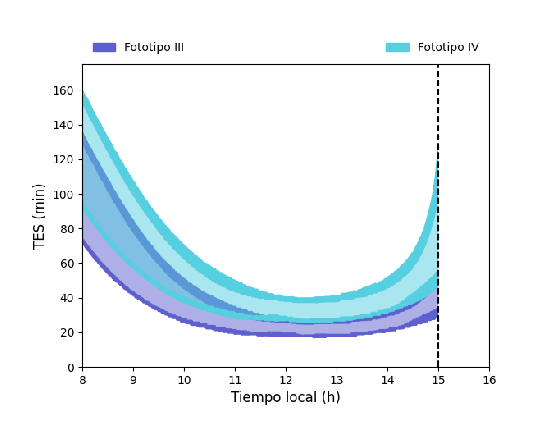
\includegraphics[scale=1.3]{images/FillDosis2.eps}
    \label{fig:dosismaxima}
    \centering
    \caption{Franja de valores en las diferentes temporadas del año para \\los TES respectivos del fototipo III y IV }
\end{figure}
\textcolor{na}{I$_{UVA}$ calculada con Modelo TUV (sup). TES para acumular 1J/cm$^2$ de Dosis$_{UVA}$ y 210 J/m$^2$ de Dosis$_{erit}$ comenzando las 11:00 hs TL; funciones mínimas y máximas con coeficientes promedios anuales en el periodo 2015-2018 (inf).}
\changefontsizes{12pt}
\begin{center}
\begin{shaded}
\changefontsizes{12pt}
\textbf{\textcolor{na}{Conclusiones}}
\end{shaded}
\end{center}
\begin{center}
\begin{shaded}
\textbf{\textcolor{na}{Referencias}}
\end{shaded}
\end{center}
\end{multicols}
\end{document}